\documentclass[UTF8]{ctexart}
\usepackage{graphicx}
\usepackage{amsmath}
\pagestyle{plain}   
% \usepackage{booktabs}
% \usepackage{subfigure}
\usepackage{setspace}
\date{}
\title{KMP算法与蛮力算法的对比实验报告} 
\author{杨景凯}
\date{2021/5/5} 
\begin{document} 
% \maketitle 
\begin{center}
    \quad \\
    \quad \\
    \quad \\
    \vskip 3.5cm
    \heiti \zihao{1}KMP算法与蛮力算法的对比实验报告\\
\end{center}
\vskip 3.5cm
\begin{quotation}
    \songti \fontsize{30}{30}
    \doublespacing
    \par\setlength\parindent{12em}
    \quad 
\begin{center}
    %学\hspace{0.61cm} 院:\underline{电子信息与电气工程学院}

    学生姓名:\underline{\qquad    \quad \quad 杨景凯    \quad  \quad\qquad }

    学\hspace{0.61cm} 号:\underline{\quad \quad\quad520021910550\quad\quad}

\end{center}
    
    \centering
    2022年5月5日
\end{quotation}
\clearpage
\tableofcontents
\clearpage
\section{实验介绍}
本次实验的目的是测试KMP算法相比蛮力算法是否更高效。为了完成实验,我选取了以下数据:
\begin{itemize}
    \item 字符串数据:总共四组字符串,长度分别为10000、100000、1000000、10000000。每组字符串为3种。
    \item 模式串数据:总共三组模式串,长度分别为10、100、1000。
    \item 字符数据:总共有三种字符,分别为'a'、'b'、'c'。
\end{itemize}
\clearpage
\section{实验结果}
\subsection{模式串长度为10}
\subsubsection{数据表格}
\begin{table}[h]
    \centering
    \begin{tabular}{|c|c|c|c|c|}
        \hline
        10&	10000&	100000&	1000000&	10000000\\
        \hline
        KMP算法&	0&	0.333333&	0.333333&	0.333333\\
        \hline
        蛮力算法&	0.333333&	0.333333&	0.333333&	0.333333\\
        \hline
    \end{tabular}
    \caption{模式串长度为10数据表格}
\end{table}
\subsubsection{数据图像}
\begin{figure}[h]
    \centering
    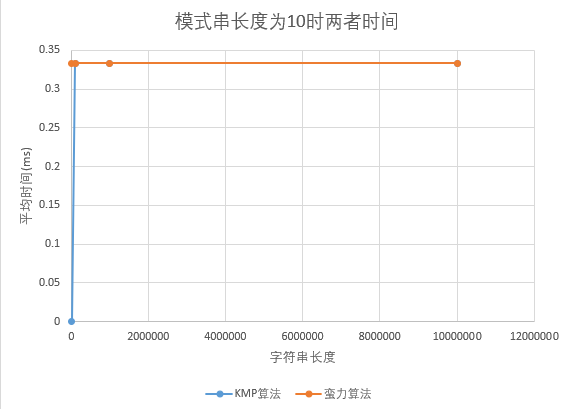
\includegraphics[scale=0.6]{10.png}
    \caption{模式串长度为10数据图像}
\end{figure}
\clearpage
\subsection{模式串长度为100}
\subsubsection{数据表格}
\begin{table}[h]
    \centering
    \begin{tabular}{|c|c|c|c|c|}
        \hline
        10&	10000&	100000&	1000000&	10000000\\
        \hline
        KMP算法&	0.333333&	1&	10.333333&	95.666667\\
        \hline
        蛮力算法&	0.333333&	1.333333&	11&	103.666667\\
        \hline
    \end{tabular}
    \caption{模式串长度为100数据表格}
\end{table}
\subsubsection{数据图像}
\begin{figure}[h]
    \centering
    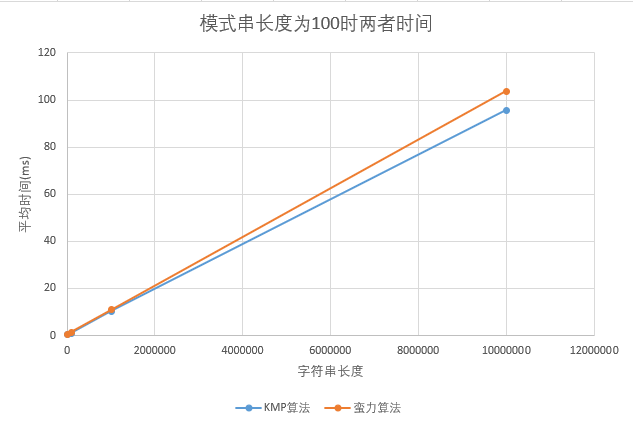
\includegraphics[scale=0.6]{100.png}
    \caption{模式串长度为100数据图像}
\end{figure}
\clearpage
\subsection{模式串长度为1000}
\subsubsection{数据表格}
\begin{table}[h]
    \centering
    \begin{tabular}{|c|c|c|c|c|}
        \hline
        10&	10000&	100000&	1000000&	10000000\\
        \hline
        KMP算法&	0.333333&	1&	11&	    96\\
        \hline
        蛮力算法&	0.333333&	1&	12.666667&	103\\
        \hline
    \end{tabular}
    \caption{模式串长度为1000数据表格}
\end{table}
\subsubsection{数据图像}
\begin{figure}[h]
    \centering
    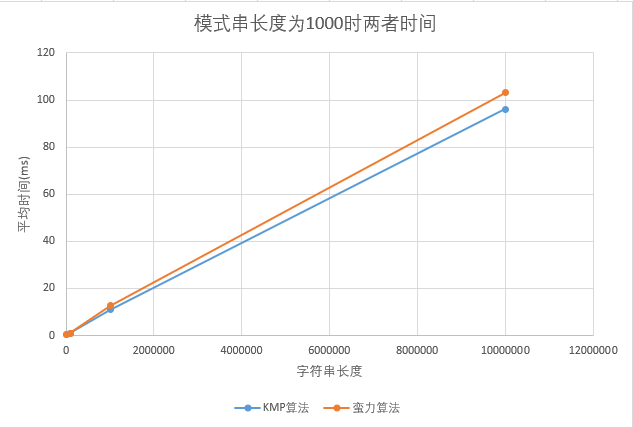
\includegraphics[scale=0.6]{1000.png}
    \caption{模式串长度为1000数据图像}
\end{figure}
\section{分析}
观察上述数据可以发现,在所有结果中,KMP算法均比蛮力算法优秀。

在实际情况中,在大多数情况下,KMP算法要比蛮力算法优秀,但是KMP算法要进行额外的建立next数组的过程,因此可能在模式串较小数据量条件下产生性能偏差的情况。

正如模式串长度为10的情况,两者几乎没有任何差别,都能很快速地计算得到结果。

\end{document}
